\section{Background}
\label{sec:background}

\subsection{Meteorological Background}

You need to find some sources indicating weather convective or frontal precipitation is the main source of extreme precipitation on the different durations. 

Explain convention and what generally causes the most extreme precipitation on the different durations. Present some typical precipitation values at the selected durations values?

Explain why the time periods of the modelled data and the observations do not have to mach exactly. 

Maybe the GEO4902 work can be included here in the background? Or it can be included as a separate section to highlight problems with forecasting extreme events? This can also be used to justify why we have to choose the maximum values from multiple grid.boxes around the respective station.   
one paper under AROME folder also highlights what effect horizontal resolution have on extreme precipitation. 

\subsubsection{Precipitation}
precipiation formation processes: collision and coalecence, ice crystal, cloud seeding. Convective, frontal, orographic. Stbility. Summer and winter. 
Precipitation is often categorized by the physical process creating it and may vary on both spatial and temporal scale. One can often relate the precipitation process to the relationship between the vertical and the horizontal extent, where the vertical velocity can be related to these two. The temporal scale varies from minutes to days, and the the spatial scale varies from hundreds of meters to hundreds of kilometers. Large-scale precipitation events are typically on a synoptic scale, characterized by a horizontal dimension many times greater than the vertical extent. Hence, the vertical velocity is often small in theses systems. Smaller-scale systems have shorter horizontal extent and often vertical extent equal to or almost equal to the vertical. In these systems the vertical speed is often large compared to large-scale systems. Normally precipitation is separated into three main categories; stratiform, orographic and convective precipitation.

\subsubsubsection{Large-scale}
some on this? at least mention somewhere what types of precipitation events usually causes the largest extremes for differnt durations. From 0-3 hours its typically convective precipitation, but when you are getting closer to a full day it might as well be large-scale stratiform precipitation. 
\subsubsubsection{orographic}
some on this?
\subsubsubsection{Convective Precipitation}
Convective precipitation originates from clouds driven by convection. These clouds are cumulus-type clouds forming in an unstable atmosphere as warm air rises due to buoyancy forces. The vertical extent is determined by the depth of the unstable layer and its degree of instability. The cumulus clouds are distinct in their shape with a flat base and a "cotton-like" appearance. They can also be observed with narrow, towering plumes on top. Horizontally the extent is typically around 3 km, while the initial thermal in which condensation first occurs can be only tens of meters. Typically the lifetime of cumulus clouds are from a few minutes to hours. If the persist for many hours they also tend to grow substantially in size. The horizontal and vertical extent is comparable, but a cumulus cloud can under right conditions (\textbf{do i need to elaborate further on this?}) develop to a cumulonimbus cloud reaching all the way to the top of the stratosphere \cite{rogers}. Once the recognizable anvil-shaped cumulonimbus is formed it is very likely to produce rain, thunder and lightning. Although cumulus clouds are commonly associated with nice weather, as the convection it self typically occurs due to the sun heating the ground during daytime in summer creating buoyant air, once the rising parcel of air becomes saturated condensation will occur and precipitation will form. As the warm and moist air rises it cools to the point where the air is saturated on water vapour. Once condensation begins, latent heat is released and precipitation forms.

maybe include some schematics on buoyancy and instability? also the dry and wet adiabat and stability criteria? 

\begin{figure}[hbt!]
    \centering
    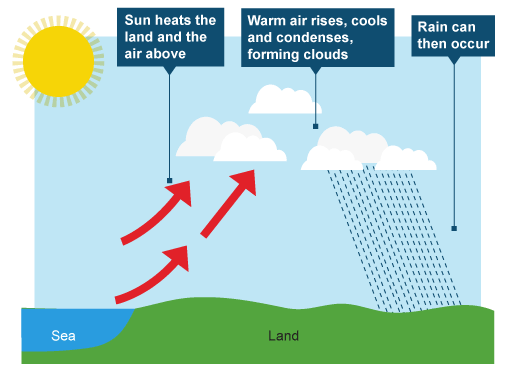
\includegraphics[scale=0.4]{figures/convection-rain.png}
    \caption{Schematic Convection. From: https://anessoriginal.wordpress.com/elective-geog/variable-weather-and-changing-climate-a-continuing-challenge/key-question-1-wc/1-convectional-rain/.
    \cite{convection}}
    \label{fig:convection}
\end{figure}


Given the short temporal scale and the small horizontal scale the convective precipitation, also known as showers, are rather local phenomena you can watch form and propagate past your neighbourhood. Events at such small scales proves hard to capture for climate models, and even operational forecasting are far from spot on with predicting the where and the when of these events. 

\begin{figure}[hbt!]
    \centering
    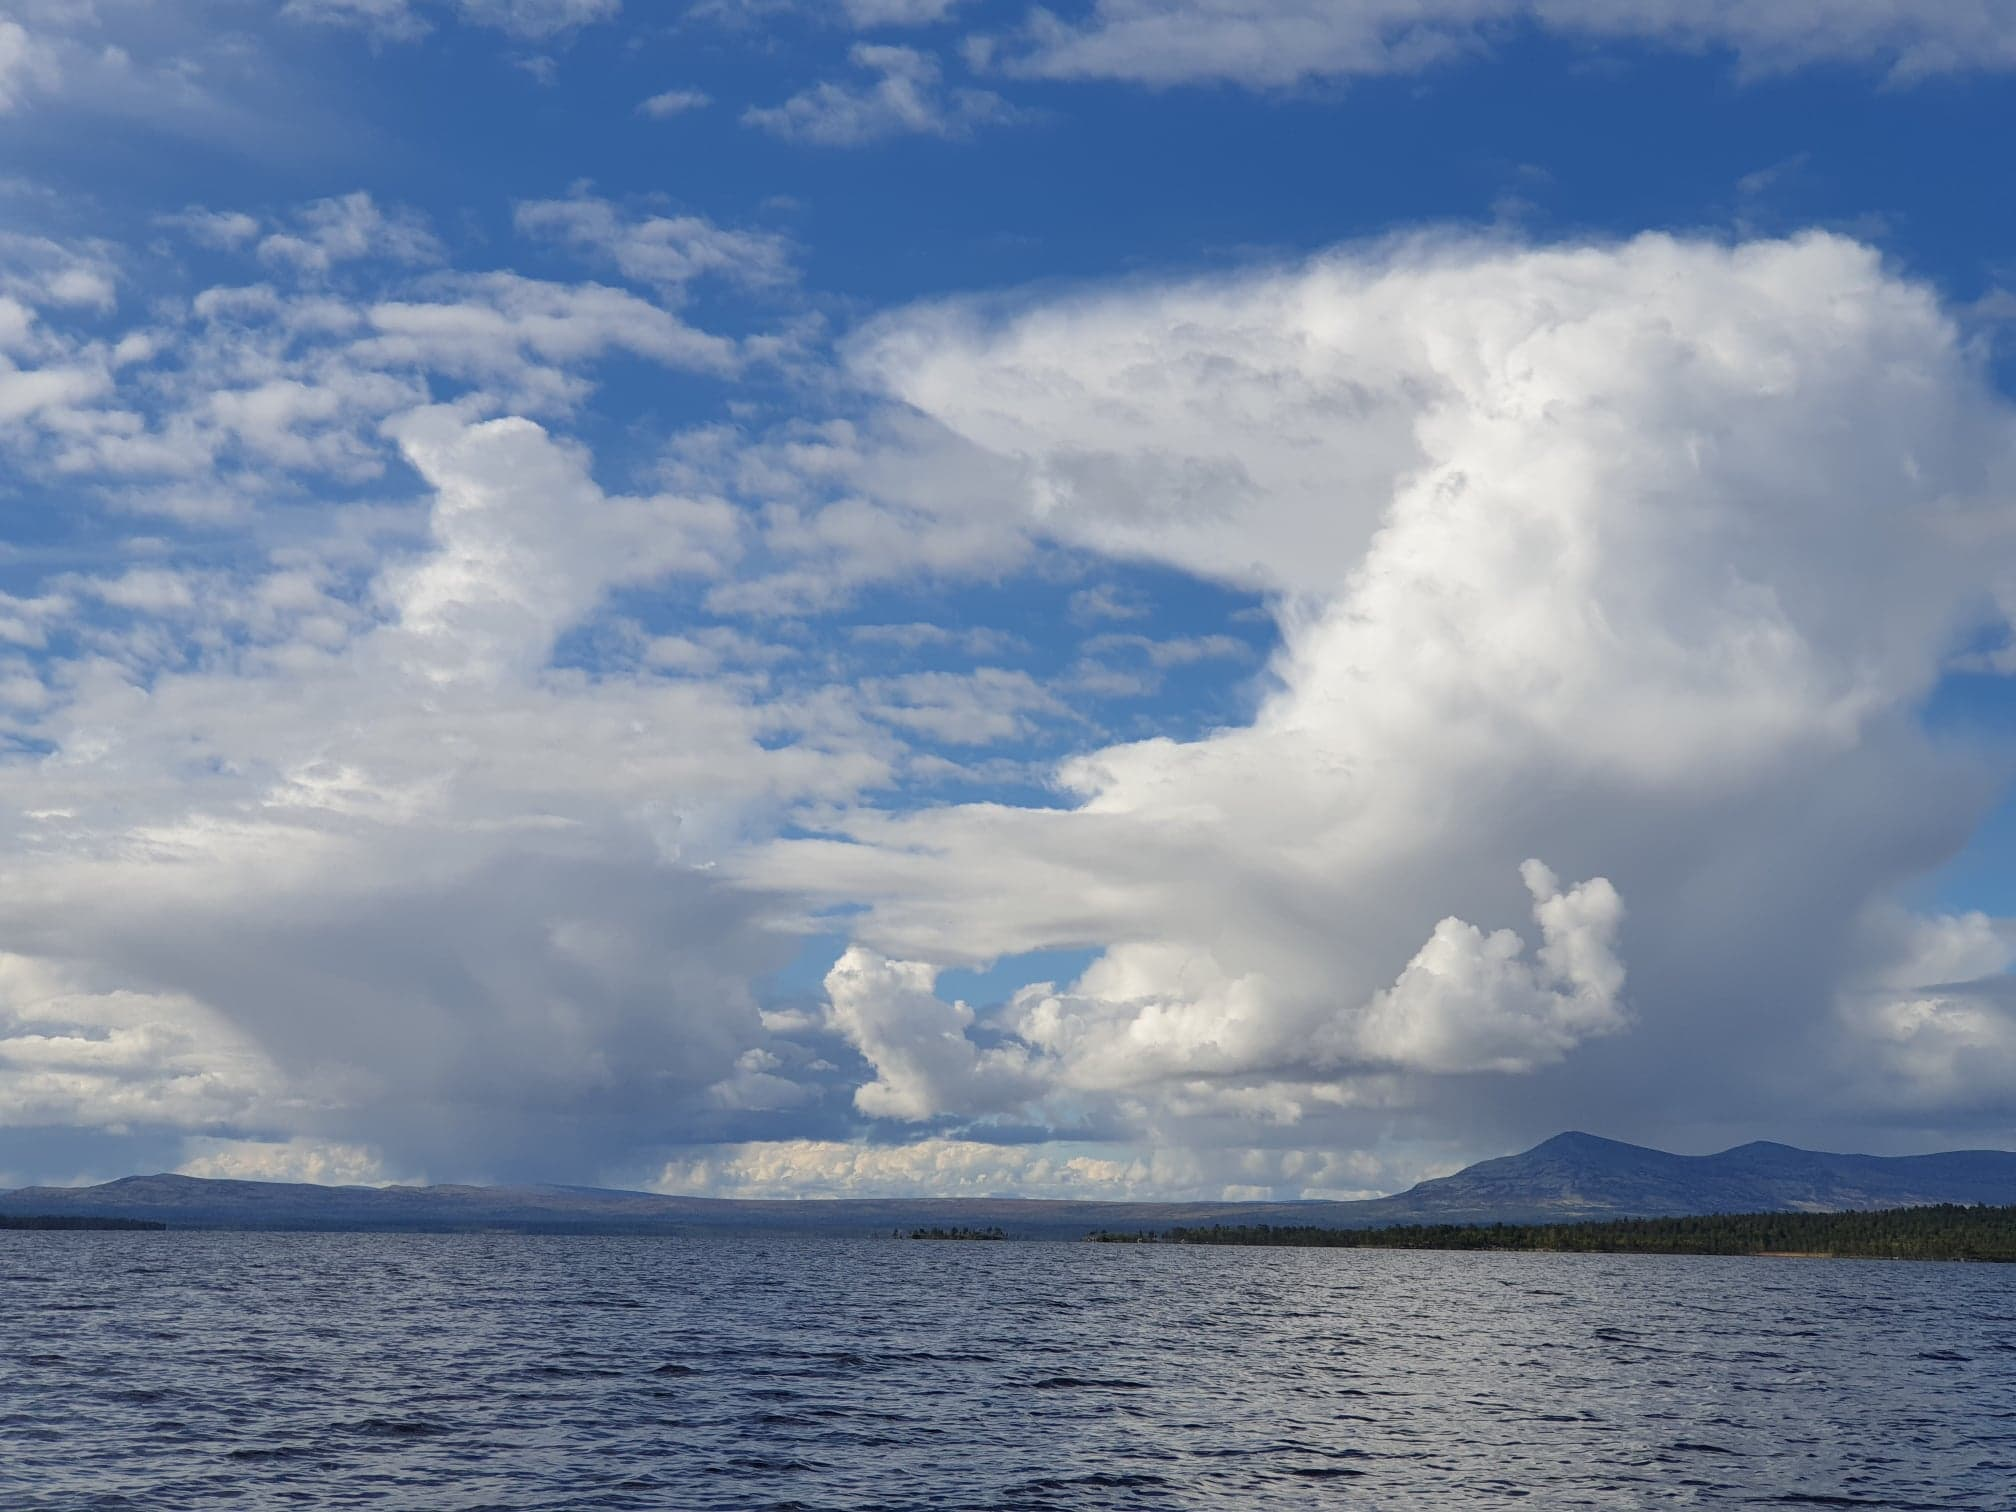
\includegraphics[scale=0.2]{figures/cumulus_bilde.jpg}
    \caption{Formation of convective Cumulus clouds over land in Femundsmarka, Norway.
    \cite{cumulus}}
    \label{fig:cumulus}
\end{figure}

\subsubsection{Convection}

\subsubsection{Dry convection}

Convection is often treated as an adiabatic process. This is a thermodynamic process in which no heat or mass is transferred between the system in question and the surroundings. However, energy can be transferred from the system to the surroundings through work. Being a compressible fluid the density of the atmosphere is a function of both temperature and pressure; $\rho = \rho(p,T)$. Furthermore it obeys the perfect gas law, and $\rho = p/RT$. As a parcel rises from an initial height $z_1$ it moves into an environment of lower pressure at height $z_2$, adjusting to this pressure by expanding along the way. This expansion exerts work on the environment, making the parcel cool. To determine the buoyancy of the parcel at $z_2$ one must know the evolution of the parcel temperature between $z_1$ and $z_2$.

Considering a parcel of ideal gas of unit mass with a volume V. Using the first law of thermodynamics,

\begin{equation}
    \delta Q = dU + dW
    \label{1law}
\end{equation}
where $\delta Q$ is an amount of heat exchange with the surroundings, $dU$ is the change in energy and $dW$ is the change in external work. Eq. \eqref{1law} can be written as 

\begin{equation}
    \delta Q = c_vdT + pdV
    \label{1law2}
\end{equation}

where $c_cdT$ is the change in internal energy due to change in temperature $dT$ and $pdV$ is the work done by the parcel on its surroundings by expanding an amount $dV$. $c_v$ is specific heat at constant volume. Rewriting Eq. \eqref{1law2} with repeated use of $p=\rho RT$ yields 

\begin{equation}
    \delta Q = c_pdT - \frac{dp}{\rho}
    \label{thermo1}
\end{equation}

where $c_p = R + c_v$ is specific heat at constant pressure. 

For adiabatic processes $\delta Q = 0$, thus

\begin{equation}
    c_pdT = \frac{dp}{\rho}
    \label{dq0}
\end{equation}

The hydrostatic balance,

\begin{equation}
    \frac{\partial p}{\partial z} +g\rho = 0
\end{equation}

describes how pressure decreases with height in proportion with the weight of the overlying atmosphere. Using the hydrostatic equation and assuming $p \simeq p_{e}$, for a small upward displacement in Eq.\eqref{dq0} the parcel`s temperature under an adiabatic displacement will change according to

\begin{equation}
    \frac{dT}{dz} = -\frac{g}{c_p} = - \Gamma_d
    \label{drylaps}
\end{equation}

where $\Gamma_d$ is called the dry adiabatic lapse rate and the notation $e = environment$. Now if the parcel is displaced from $z_1$ to $z_2$ it will experience a restoring force depending on the density of the environment. At $z_2$ the environment has temperature $T_2 \simeq T_1 + (dT/dz)_e \delta z$ where $(dT/dz)_e = \Gamma_e$ is the environmental lapsrate, pressure $p_2$ and density $\rho_2 = p_2/RT_2$. The parcel has temperature $T_P = T_1 - \Gamma_d\delta z$, pressure $p_2$ and density $\rho_P = p_2/RT_P$. Depending on whether $T_P$ is greater than, equal to or less than $T_2$ the parcel will be positively, neutrally or negatively buoyant. Thus, criterion for stability can be written

\begin{equation}
    \begin{rcases}
      \text{Unstable}\\
      \text{Neutral}\\
      \text{Stable}
    \end{rcases}   
    \text{if} \left(\frac{dT}{dZ}\right)_e = \Gamma_e 
    \begin{cases}
      < - \Gamma_d \\
      = - \Gamma_d \\
      > - \Gamma_d
    \end{cases}
    \label{stabcond}
\end{equation}
\textbf{or according to CLOUD: ALSO CHECK $\GAMMA_e$ in the above. also, include a figure on this}
\begin{equation}
    \begin{rcases}
      \text{Stable}\\
      \text{Neutral}\\
      \text{Unstable}
    \end{rcases}   
    \text{if} \left(-\frac{dT}{dZ}\right)_e 
    \begin{cases}
      < \Gamma_d \\
      = \Gamma_d \\
      > \Gamma_d
    \end{cases}
\end{equation}

\begin{equation}
    \begin{cases}
        \Gamma = \Gamma_d \\
        \gamma = \Gamma_e
    \end{cases}
\end{equation}

From Eq. \eqref{stabcond} a compressible atmosphere is unstable if temperature decreases with height faster than the adiabatic laps rate. Given $c_p = 1005 Jkg^{-1}K^{-1}$ in Eq. \eqref{drylaps} $\Gamma_d \simeq 10 K km^{-1}$. Typically the dry laps rate decreases from around 6,5 $K km^{-1}$ at low latitudes to around 4.5 $K km^{-1}$ at polar latitudes \ref{lapsrate}. Thus, no dry convection is expected and the atmosphere can generally be considered stable to dry convection.     

\textbf{must describe the unknowns where they are first mentioned}

\subsubsubsection{Moist convection}

Since the atmosphere is normally stable in the absence of condensation most convection in the atmosphere is moist convection. If a moist air parcel is lifted it cools adiabatically, and if it is cooled enough to saturate some water vapor condenses to form a cloud. Once saturated to parcel releases latent heat, adding buoyancy to the parcel and thus increasing the instability.
Moisture of air is often expressed as specific humidity 

\begin{equation}
    q = \frac{\rho_v}{\rho}
\end{equation}

This is the ratio of mas of water to the mass of air er unit volume. Q is conserved given no mixing. The saturation-specific humidity, $q_*$, is the specific humidity at which saturation occurs. $q_*$ can be written:

\begin{equation}
    q_* = \frac{\frac{e_s}{R_v T}}{\frac{p}{RT}} = \left(\frac{R}{R_v}\right)\frac{e_s}{p}
    \label{qnote}
\end{equation}

where $e_s$ is saturated partial pressure of water vapor. 

Implicitly this means that $q_*$ is a function of both temperature and pressure. Lifting a parcel would decrease the pressure and cool the parcel. This alone would make q* increase with altitude, but the exponential dependence of es on T counteracts this effect, making the q* decrease rapidly with altitude. Thus a moist parcel usually do not have to rise a lot before it reaches the condensation level Zc where $q>q_*$. At this point and above excess water vapor will condensate creating a visible cloud. The cloud will extend up in the atmosphere until neutral buoyancy. As the parcel rises latent heat is released, resulting in a slower decrease of temperature with height compared to the dry adiabatic as rate.  Thus, a warmer or moister air parcel will result in a taller cloud compared to drier or cooler air. While the temperature of the parcel changes according to the dry adiabatic laps rate below the cloudbase, it follows the saturated adiabat upwards from $z_c$. 

When condensation occurs there will be a release of latent heat in the amount $\delta Q = -L dq$ where $L$ is latent heat of condensation and $dq$ is change in specific humidity $q$. For an air parcel undergoing moist adiabatic displacement one can insert this into \eqref{thermo1} to get 

\begin{equation}
    c_p dT = \frac{dp}{\rho}-L dq
    \label{adlap}
\end{equation}

Assuming hydrostatic balance of the environment, $dp/\rho = -gdz$ gives

\begin{equation}
    d(c_pT + gz + Lq) = 0
\end{equation}

where $c_pT+gz$ is the dry static energy and $Lq$ is the latent heat content. Combined these two terms are called the moist static energy. Furthermore, since the parcel is always saturated $q$ can be replaced by $q_*$ in Eq.\eqref{adlap}, and since $q_*=q_*(p,T)$ now

\begin{equation}
    dq_* = \frac{\partial q_*}{\partial p}dp + \frac{\partial q_*}{\partial T}dT
    \label{dqnote}
\end{equation}

Inserting Eq. \eqref{qnote} in Eq. \eqref{dqnote} yields 

\begin{equation}
        \frac{\partial q_*}{\partial p} = -(\frac{R}{R_v})\frac{e_s}{p^2} = -\frac{q_*}{p}
        \label{qfracp}
\end{equation}
and
\begin{equation}
            \frac{\partial q_*}{\partial T} = (\frac{R}{R_v})\frac{1}{p}\frac{de_s}{dT} = (\frac{R}{R_v})\frac{\beta e_s}{p} = \beta q_*
            \label{qfracT}
\end{equation}

where $\beta e_s = de_s/dT$. Combining Eq. \eqref{qfracp}, Eq. \eqref{qfracT} and Eq. \eqref{adlap} with some rearranging yields

\begin{equation}
    -\frac{dT}{dz} = \Gamma_s = \Gamma_d \left[\frac{1+Lq_*/RT}{1+\beta Lq_*/c_p} \right]
\end{equation}

$\Gamma_s$ is called the saturated adiabatic lapse rate. The term inside the brackets are always less than unity, making $\Gamma_s < \Gamma_d$. However, at high latitudes $q_*$ becomes very small, making them close to equal. The qualitative impact on condensation is evident; release of latent heat within a rising parcel makes it warmer and thus more buoyant, destabilizing the atmosphere, that is if

\begin{equation}
    -(\frac{dT}{dz}) < \Gamma_s
\end{equation}

where $\Gamma_s < \Gamma_d$ \cite{marshall} \textbf{this is not consistent with the below}. 

Thus the stability criteria for moist air is \textbf{make sure the following is consistent with the above. from two different sources. not sure its consistent now! but the writing under the following is correct and consistent with the figure.}

\begin{equation}
\begin{gathered}
    \text{Absolutely stable} (-\frac{dT}{dZ})_e < \Gamma_s \\
    \text{Saturated neutral} (-\frac{dT}{dZ})_e = \Gamma_s \\
    \text{Conditionally unstable} \Gamma_s < (-\frac{dT}{dZ})_e < \Gamma_d \\
    \text{Dry neutral} (-\frac{dT}{dZ})_e  = \Gamma_d \\
    \text{Absolutely unstable} (-\frac{dT}{dZ})_e > \Gamma_d
    \label{moist_stability}
\end{gathered}
\end{equation}

Once a saturated parcel is displaced upwards its temperature will decrease according to the pseudoadiabatic laps rate. If the environmental laps rate is greater (more negative) than $\Gamma_d$ the parcel will be warmer than the surroundings and hence accelerate in the direction of the initial displacement. If the environmental laps rate is smaller (less negative) than $\Gamma_s$ the parcel will be colder than the surroundings and hence accelerate in the direction opposite of the the initial displacement. This stability criterion is illustrated in Figure \eqref{fig:stability}. According to \eqref{moist_stability}, an important difference between moist and dry air is that initially stable moist air may be absolutely unstable or conditionally unstable if lifted.  

\begin{figure}[hbt!]
    \centering
    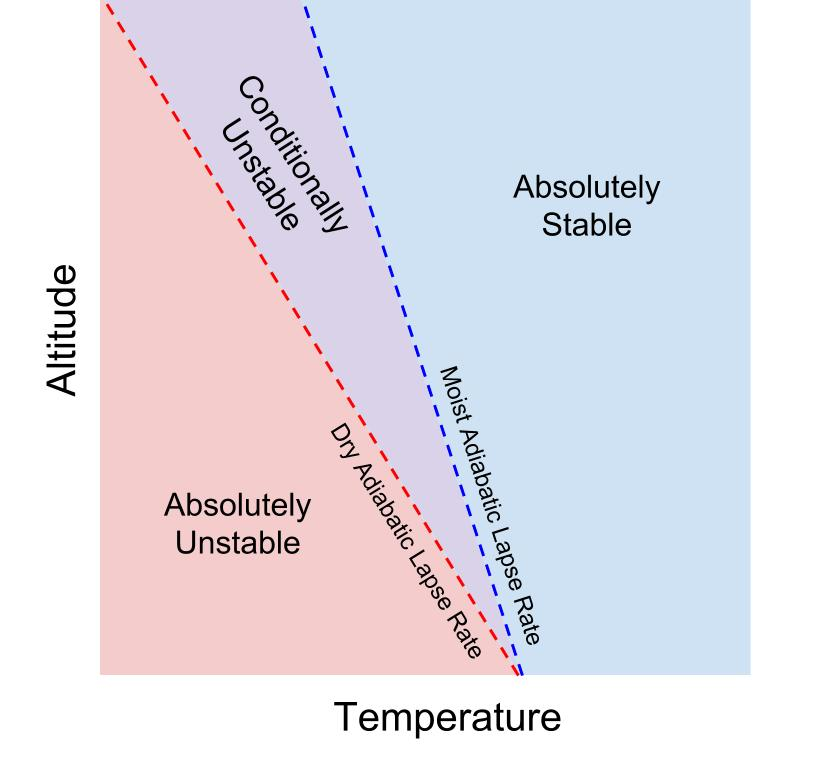
\includegraphics[scale=0.3]{figures/stability_criterie.jpg}
    \caption{Stability criteria from \url{http://pressbooks-dev.oer.hawaii.edu/atmo/chapter/chapter-5-atmospheric-stability/}}
    \label{fig:stability}
\end{figure}

\textbf{maybe include some info on CCL and LCL here?}

\subsubsection{Types and location of convection}

\subsection{Non-stationarity}
\url{https://agupubs.onlinelibrary.wiley.com/doi/full/10.1002/2016GL072201} \\
\url{https://www.researchgate.net/publication/262535997_RainIDF_Automated_derivation_of_rainfall_intensity-duration-frequency_relationship_from_annual_maxima_and_partial_duration_series} \\
\url{https://www.sciencedirect.com/science/article/pii/S2212096317300165} \\
\url{https://www.nature.com/articles/srep07093}


\subsection{Area}

The area investigated in this thesis is Oslo, the capitol of Norway. This location is selected for a number of reasons. Firstly there are multiple stations in the area witch have long, high quality data series of precipitation. This is essential because it allows for comparison to the modeled IDF values. When analysing IDF curves short time series is a problem in it self, therefore having multiple high quality data series is very valuable to the analysis. Also, multiple stations covering a rather small area like in this case may highlight certain features in the IDF curves related to topography or other mechanisms influencing precipitation that would otherwise have been hidden. Secondly the Oslo area is a typical urban area, making it vulnerable to short duration extreme precipitation. Improving the knowledge on extreme precipitation events may potentially save the area and its population for large weather-related costs in the future. Another reason for selecting this area was the availability of processed data. Data from the selected stations had been cleaned and checked for analysis beforehand as part of the \textbf{Julia paper (how do I address this?)}. 

\subsection{Data}
\subsubsection{Measurements}
Precipitation measurements used in this project is obtained from pluviometers operated by the Norwegian Water Resources and Energy Directorate (NVE) or the respective municipalities in corporation with  MET Norway. Since the late 1990s and early 2000s the operating pluviometer has been the Lambrecht 1518H3 tipping bucket pluviometer manufactured by the German company Lambrecht meteo GmbH \cite{lutz_idf}. The Lambrecht pluviometer has a measuring range of 0.1 mm precipitation at time resolution of 1 minute and a given accuracy of $\pm$ 2$\%$. Intensity correction is done to account for loss of rain due to the time required for the bucket to tip. MET Norway supervised the installation of the pluviometers and ensured installation according to the recommendations from the World Meteorological Organization (WMO). Additionally MET Norway performed quality control and storage on all data from the pluviometers. Before the now operational Lambrecht some of the stations operated with the Norwegian produced pluviograph Plumatic, manufactured by Kongsberg Våpenfabrikk A/S. It was replaced partially due to is lack of heating, making it operational only in the extended summer months, from mid-April to mid-October. The Lambrecht also suffers from poorer data quality during winter due to snowcaps or ice-slush obstruction spite been heated.  

The proposed method in this study requires annual maxima for each duration as input, thus a requirement for season completeness is necessary. The requirement where here set to at least 80\% of the days throughout the season covered and of good quality. Hence the precipitation series extracted where shorter than the total operational period for all stations. The number of extracted years with annual maxima is found in Table \textbf{number of table below}. Lutz et al 2020 analysed monthly precipitation for 1,2 and 3 hours in two locations in Oslo and found that the highest occurrence of short-duration, high-intensity precipitation was during the summer months. In combination with lack of high-quality data during the winter period, especially from before the 1990s when the Plumatic pluviometer were still in use, makes the extended summer period, 1st of May to 30th of September, best suited for the IDF analysis in this study. Furthermore, time series of 10 years is here considered to be an absolute minimum for calculation of IDF values. The twelve stations listed in Table \textbf{table under, need numer} are the ones left meeting these criteria in the municipality of Oslo.   

\\

\begin{center}
\begin{tabular}{ |p{3cm}||p{3cm}|p{3cm}|p{3cm}|  }[hbt!]
\hline
\multicolumn{4}{|c|}{Oslo Stations} \\
\hline
 Station Name & Station NR & Years AM & Operational From\\
 Ljabruveien & 17980  & 17 &  01.01.1985-\\
 Lambergseter & 18020 & 25 & 15.05.1999-\\
 Hovin & 18210 & 17 & 15.01.1999-\\
 Haugenstua & 18269 & 15 & 01.01.2000-\\
 Vestli & 18270 & 32 & 18.04.1974-\\
 Hausmannsgt & 18320 & 20 & 21.06.1984-04.11.2013\\
 Disen & 18420 & 20 & 02.06.1998-\\
 Vestre Vika & 18640 & 13 & 22.05.1974-03.10.1998\\
 Blindern PLU & 18701 & 48 & 16.04.1968-\\
 Bygdøy & 18815 & 16 & 01.01.2000-\\
 Besserud & 18920 & 13 & 29.09.2998-\\
 Lilleaker & 18980 & 13 & 01.01.2000-   
\end{tabular}
\end{center}

\textbf{the section "measurements" in Lutz et al., 2020 has the description of the station data. Essentially annual maxima for each duration and station.} Tipping bucket pluviometers does not function properly during winter, so this is basically summer-data. Time series of 10 years is concidered an asolute minimum here, hence the choice of these 12 stations (you can also include the two from Bærum if you get the data). 

\subsubsection{AROME model and data}

% - HCLIM is the regional climate version of HARMONIE.
% - HCLIM uses HARMONIE-AROME for convection-permitting modelling.
% - HARMONIE-AROME is the ALADIN-HIRLAM (new name for this is now ACCORD) implementation of AROME physics within the HARMONIE model system.
% - HARMONIE-AROME is used in operational forecasting in MetCoOp (possibly to be called UWC-East from 2022) by MET Norway, SMHI, FMI, and from 2022 the Baltic countries.
% - AROME is a separate model system developed by MeteoFrance, but it is not what is run in Norway.
For this study precipitation output from the HCLIM38 model has been used.
The atmospheric model HARMONIE-AROME uses the atmospheric physics from Applications of Research to Operations at Mesoscale (AROME) (Seity et al. 2011)\cite{seity_arome} model, developed by Météo-France. The physics package is designed for convection-permitting scales and non-hydrostatic dynamics with 65 vertical layers and 3 km horizontal resolution (Bengtsson et al. 2017)\cite{bengtsson_arome}. HARMONIE-AROME is used for operational high-resolution numerical weather prediction (NWP) in the cooperative effort named Meteorological Cooperation on Operational Numerical Weather Prediction (MetCoOp) between the Norwegian Meteorological Institute (MET-Norway), the Swedish Meteorological and Hydrological Institute (SMHI) and the Finnish Meteorological Institute (FMI) (Müller et al. 2017)\cite{muller}. Recently HARMONIE-AROME has been used in a regional climate-configuration called HARMONIE-Climate cycle 38 (HCLIM38) for long-term climate simulations (Lind et al. 2020)\cite{lind_arome]}. Being one of the first long-term climate simulations on regional convection-permitting (\<4km) scales with explicit deep convection for the Scandinavian region(Lindstedt et al. 2015\cite{lindstedt_hclim}; Lind et al. 2016\cite{lind_hclim}), this data-set provides added opportunities for analysis of extreme precipitation. A comprehensive description of the model system is presented in Belušić et al.(2020)\cite{belusic_hclim}. 

\textbf{it would be nice with a figure shoeing the model system structure..}
\\
\\
\textbf{this paragraph might be removed. Overkill or necessary?}
HARMONIE-AROME is developed, maintained and validated through the shared ALADIN-HIRLAM system, a collaboration of 26 countries on short-range mesoscale NWP. The international research program High Resolution Limited Area Model (HIRLAM) was initiated in 1985 and consists of the National Meteorological Services (NMSs) from 10 countries. Similarly Aire Limitée Adaptation Dynamique Développement International (ALADIN) is a collaboration among 16 central-European NMSs. HARMONIE-AROME is the ALADIN-HIRLAM implementation of the AROME physics within the HARMONIE model system. The focus of the HIRLAM colaboration in recent years has been on the convective-permitting scale and thus to adapt HARMONIE-AROME for use in the common ALADIN-HIRLAM NWP system for accessibility for all collaboration members (Bengtsson et al. 2017)\cite{bengtsson_arome}.
\\
\\
The model dynamics of HARMONIE-AROME is based on the fully compressible Euler equations \textbf{source on Euler. Simmons and Burrige 1981?)}. At 2.5-km resolution deep convection is expected to be resolved explicitly, hence the model has no deep convection parameterization. Shallow convection on the other hand is parameterized though a mass-flux framework consisting of updrafts and thus transport of heat, momentum and moisture(Bengtsson et al. 2017)\cite{bengtsson_arome}. Eddy diffusiveity is parameterized through a turbulence scheme called HARATU. \textbf{Note to self: for more info on the (dual) mass flux read the article in detail}. The surface physics is simulated by the SURFEX surface scheme \textbf{source on SURFEX}. SURFEX simulates surface aerosols, chemistry processes and other surface variables. Each surface grid box is represented by four tiles: sea or ocean, lakes, urban areas and nature (soil and vegetation), where the nature-tile is further divided into patches depending on vegetation type. Energy exchange between the surface and atmosphere for the different tiles are simulated with a collection of schemes(Bengtsson et al. 2017)\cite{bengtsson_arome}. Surface topography is is based on Global Multi-resolution Terrain Elevation Data (GMTED2010) \textbf{source on GMTED2010 Danielson and Gesch 2011?}. Work is currently done to prepare the model for operational use at increased resolution (100 layers, 0.5-1.3 km). This will improve the representation of both deep and shallow convection. Additionally this work aims to result in better understanding of model behaviour in the gray zone between shallow convection and turbulence.
\\
\\

The climate setting of HARMONIE-AROME (HCLIM38) proved strong improvement on representation of precipitation compared to similar model-setups with coarser models in Lind et al. 2020 \cite{lind_arome}. Most evident was the improvement in reduction of "drizzle" and increased occurrence of high intensity precipitation events in addition to better timing and amplitude of the diurnal cycle. The simulations was conducted within the Nordic Convection Permetting Climate Projections project (NorCP), which is one of the leading projects on increasing knowledge of climate changes and processes over the Fenno-Scandinavian region. The boundary state for HCLIM38 is obtained from the global ERA-Interim reanalysis (Berrisford et al. 2011)\cite{erai}. This data has a horizontal grid of approximately 80 km, available every 6 hour. An alternative set of boundary data from the Earth System Model (ESM) EC-Earth (ECE) is also applied, providing a slightly different climate simulation (Lind et al. 2020)\cite{lind_arome}.    

Based on the seasonal forecast system of the European Centre for Medium-Range Weather Forecasts (ECMWF), the EC-Earth simulates all relevant parts of of the Earth system, including physical, chemical and biological processes. Whereas a typical GCMs simulate atmospheric and oceanic components, an ESM also includes information on a global carbon cycle, dynamic vegetation, ocean bio-geo-chemistry, atmospheric chemistry and continental ice sheets.\textbf{source: https://www.climateurope.eu/earth-system-modeling-a-definition/}. Feedback cycles are also modelled, allowing for gained information on how the climate system is reacting to certain changes like deforestation or reduced surface albedo \textbf{source: https://www.nature.com/scitable/knowledge/library/studying-and-projecting-climate-change-with-earth-103087065/}. This improves the complexity and hence the overall representation of physical processes within the system. \textbf{Arctic temperatures have a cold bias i ECE. Could this affect the precipitation patterns in Norway?}.

The ERA-Interim reanalysis is the product of a data assimilation system. It is produced using an analysis of the current state of Earth as initial conditions, blending available observations with short-range forecast to produce the next analysis. ERA-Interim is globally complete and consistent in time, making it suitable as input to climate models and applicable for a variety of studies \textbf{source: https://www.ecmwf.int/en/about/media-centre/focus/2020/fact-sheet-reanalysis}. Providing a bridge between pure observations and pure modelling, a reanalysis is designed to represent the past state of the entire climate system in the most accurate way possible. For this reason, a reanalysis is sometimes refereed to as "the truth". In contrast to ECE, ERA-Interim was found to have a positive temperature bias in the Arctic region according to \textbf{https://climatedataguide.ucar.edu/climate-data/era-interim}.  

\\
\cite{lind_arome} citation figure arome domain 
\begin{figure}[hbt!]
    \centering
    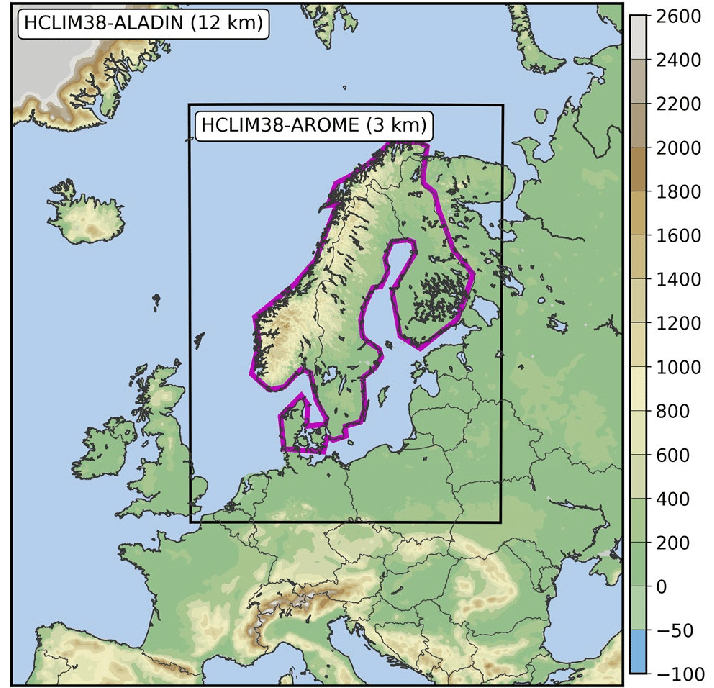
\includegraphics[scale=0.2]{figures/arome_domain.png}
    \caption{Domain used for HCLIM38-ALADIN (12km) simulation and domain used for HCLIM38-AROME (3km) simulation in the inner black rectangle. The colorscale represents the altitude above mean sea level in meters, and the magent colored area defines the Fenno-Scandinavian region. Source: Lind et al. 2020 \cite{lind_arome}}
    \label{fig:arome_domain}
\end{figure}

\subsubsection{AROME: difficulties with convective forecasting, an example}

MÜller et al. 2017 \cite{muller} highlights the challenge of precise precipitation forecasting of convective cells. Even though the precipitation amount may be well-forecasted it can be fatal for decision-makers if it is mislocated with a few kilometers. Here a case study illustrating this challenge is presented. 

7nt of August 2019 15:00-18:00 UTC a heavy rainfall event occurred in Bærum, Norway. According to a METinfo report \ref{metreport} the event caused local damage, clogged drainage systems and numerous flooded basements. The forecast prior to the event revealed unstable air masses with strong vertical movement throughout southern Norway. Besides an elevated KAPE-index north-west of where the event actually occurred there where little indication for such an event in the Bærum-area. During the event several records for short-duration precipitation was set at the Gjettum station in Bærum: 36,5mm/30min, 47,9mm/1h and 61,3/3h. These recordings have returnperiods of >200 years, >100 years and >50 years respectively. The 24-h accumulated precipitation forecast is produced as a 10-member ensemble mean. The ensemble mean forecast in Figure \ref{fig:ens_mean} show some precipitation in the area west of Bærum with magnitude of around 2 mm/24h.  

\begin{figure}[hbt!]
    \centering
    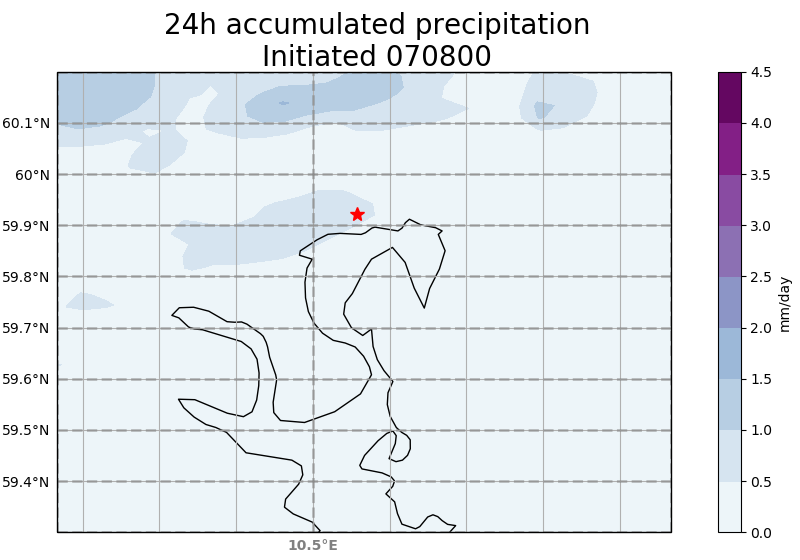
\includegraphics[scale=0.4]{figures/ens_mean.PNG}
    \caption{24-h ensemble mean precipitation forecast initiated 7th of August 2019 00:00 UTC. The black line is the shoreline in the Oslofjord, Norway. The red star marks the location of the Bærum station.}
    \label{fig:ens_mean}
\end{figure}

The small precipitation magnitude in the Figure \ref{fig:ens_mean} is due to the spatial distribution of precipitation in the 10 ensemble members. If 1 out of 10 ensemble members predict 50 mm precipitation at a certain location and the others predict 0 mm the ensemble mean amount will be very small. In reality this product can only provide information on what location the members agree precipitation will occur, and not so much the magnitude of the event itself. Ensemble members are different realizations of the model, each with a slightly different set of initial conditions. Even though the ensemble mean does not reveal any major event the individual members may provide some information on the size of the event. All members are equally a realization of the model, which highlights the uncertainty of the precipitation forecasting within AROME. In Figure \ref{fig:ensmember} two ensemble members show two very different forecasts. One, ensemble member 4, seems to capture the localization quite well, only missing with a few kilometers. The magnitude of the event is also captured quite well in this member with a maximum value of around 45-50mm/24h. While having a very different intensity from the observed at 61.3mm/3h it is still a fairly large event for the area. Shorter-duration forecasts initiated hours before the observed event did not show magnitudes anywhere close to the observed event. The other ensemble member, member 1, predicts no precipitation in the area at all within 24 hours of the forecast initiation. It should be pointed out that these are only 2 out of 10 ensemble members, used as example to highlight the potential difference between each member of one forecast.   

\begin{figure}[hbt!]%
    \centering
    \subfloat[\centering Ensemble member 1]{{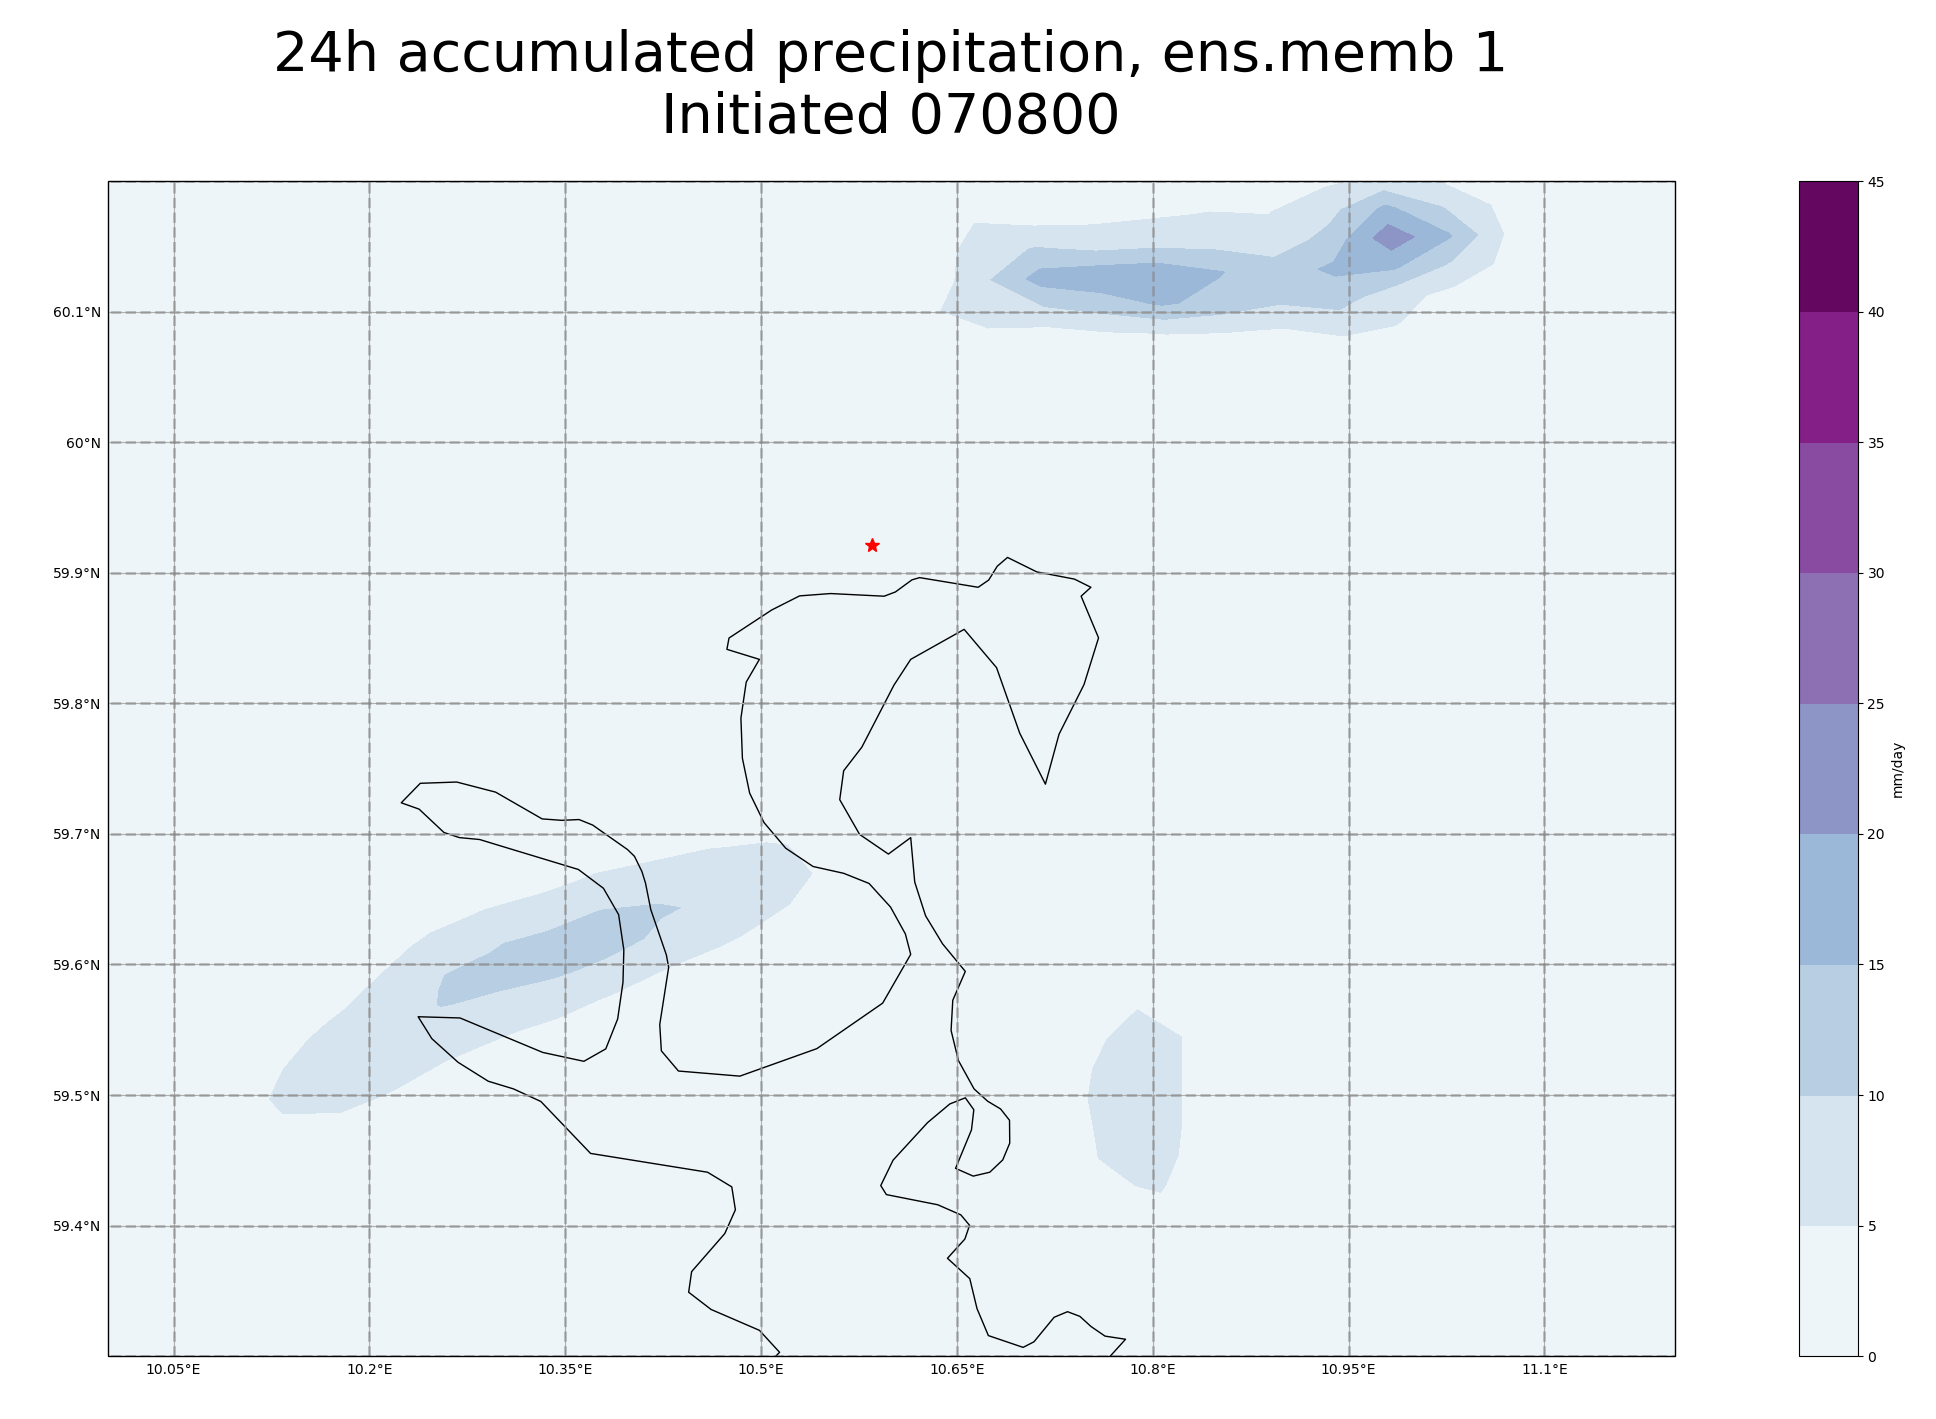
\includegraphics[width=5.5cm]{figures/ens1.PNG} }}%
    \qquad
    \subfloat[\centering Ensemble member 4 ]{{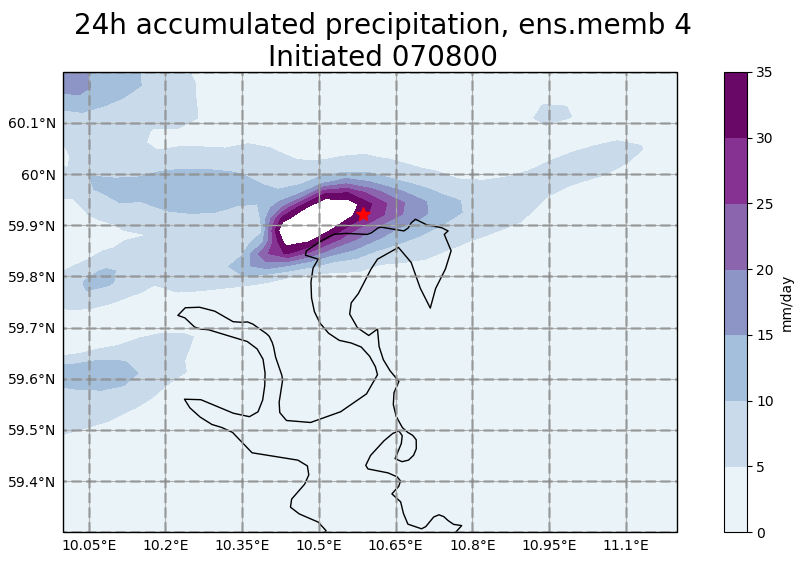
\includegraphics[width=5.5cm]{figures/ens4.PNG} }}%
    \caption{Two ensemble members from the 24-h accumulated preciptiation forecast initiated 7th of August 2019 at 00:00. The red star marks the Bærum station.}%
    \label{fig:ensmember}%
\end{figure}

Ensemble member disagreement makes decision making based on this forecast hard or impossible. It is not known whether this event was due to deep or shallow convection (\textbf{I guess shallow?}). As mentioned in Section \textbf{ref to section with AROME and deep convection} deep convection is expected to be resolved explicitly, while shallow convection is parametrized. In this case either the parametrizaion failed or the scales in action was to small to be resolved by the model. Even though progress in made within the modelling system to improve convective precipitation forecast, it is evident that state of the art forecasting system is still struggling with small-scale convection. \textbf{is this too "negative"? AROME is definitely a high-skilled model, ant at times it predicts these events quite well. Should I include an example of this in a sentence or two as well?}

This case study serves as an example of how different "realities" within the model predicts different magnitude and location of convective precipitation. It is not possible to indicate weather one ensemble member are more likely to mach observations than others. This behaviour also supports the argument in Section \textbf{section where temporal overlap obs and mod is explained} of no need for perfect temporal overlap between the observed and the modelled precipitation.       

\section{Method}

There are several ways to extract annual maxima from the precipitation data. In the following paragraph the different methods used on this study will be presented.  
\subsection{Annual Maxima}

The block maxima used in these calculations are annual maximum precipitation for durations ranging from 15 minutes to 24 hours. Since station-based data is typically used for the GEV calculation the block maxima represent a single point in space. In terms of extreme precipitation, what is this single-point measurement really representing? Is it representative for a larger area or only for the specific gridpoint? Some convective events during summer are extremely localized (with example). Showers like this might pass only a couple of kilometres away from a station, but still cause severe damage to the downstream area in which the station is located. Using gridded precipitation values from the AROME model allows for extraction of annual maximum precipitation not only from the gridpoint closest to the station, but also from multiple gridpoints surrounding the station. The idea is that including data from gridpoints around the one closest to the station may result in an analysis representative for a larger area compared to a single point. As a station potentially misses events by the smallest margin it is also challenging to know whether modelled precipitation at a gridpoint is under- or over-estimated compared to the station-based annual maxima. Here follows the four different methods used to compute the annual maximum precipitation from the 20-year data series provided by the climate setting of the AROME forecasting model. Annual maxima are extracted for each duration, making a data-series with maximum values with length n equal to number of years available (20). The raw data has temporal resolution of 15 minutes. The overall goal with these different methods is to find the method that are most consistent with the station-based annual maxima and IDF-values, but also to determine what they represent physically as it is hard to determine what the “true” extreme precipitation state of the area actually is.  

\begin{enumerate}

\item 1grid 
Hereafter named “1GRID”. Select gridpoint closest to the respective station. A sliding filter for each duration is applied, summing datapoints to the given duration length and creating a new dataset. From this time-series the annual maximum is extracted for each duration.

\begin{figure}[hbt!]
    \centering
    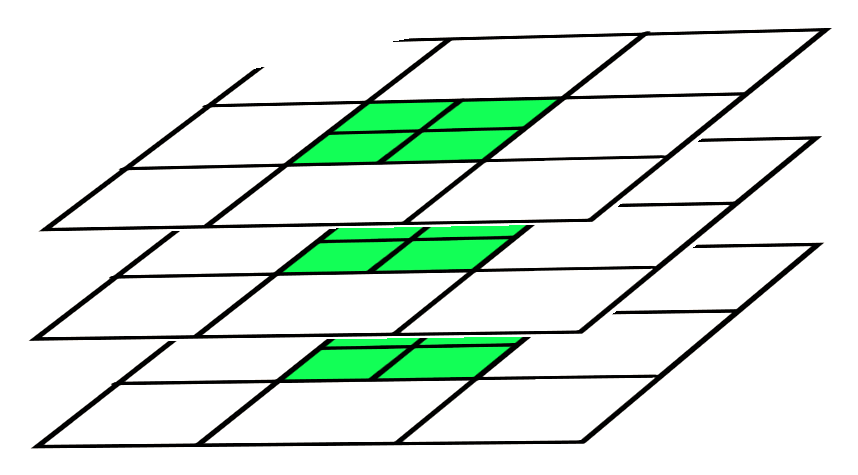
\includegraphics[width=4.5cm]{figures/met1g.PNG}
    \caption{something here about figure}
    \label{fig:my_label}
\end{figure}

\item 9grid
Hereafter named “9GRID”. Select the gridpoint closest to the respective station and the neighbouring gridpoints in a 3x3 matrix with the centre-gridpoint being the one closest to the station. A sliding filter for each duration is applied, summing datapoints to the given duration length and creating a new dataset. The filter selects the maximum value out of the 9 gridpoints for each timestep. Thus, a resulting annual maximum value for a given year and duration may consist of precipitation values from different gridpoints. 

\begin{figure}[hbt!]
    \centering
    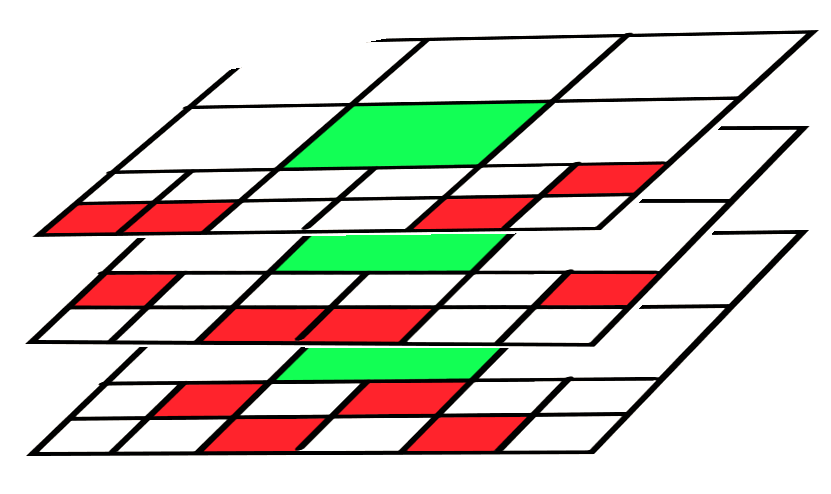
\includegraphics[width=4.5cm]{figures/met9g.PNG}
    \caption{something here about figure}
    \label{fig:my_label}
\end{figure}

\item 9mean
Hereafter named “9MEAN”. Select the gridpoint closest to the respective station and the neighbouring gridpoints in a 3x3 matrix with the centre-gridpoint being the one closest to the station. A sliding filter for each duration is applied, summing datapoints to the given duration length and creating a new dataset. The filter selects the maximum value for each of the 9 gridpoints, making 9 time-series with annual maximum values for each duration. The mean annual maximum of the 9 is then calculated for each duration.  

\item 9max
Hereafter named “9MAX”. Select the gridpoint closest to the respective station and the neighbouring gridpoints in a 3x3 matrix with the centre-gridpoint being the one closest to the station. A sliding filter for each duration is applied, summing datapoints to the given duration length and creating a new dataset. The filter selects the maximum value for each of the 9 gridpoints, making 9 time-series with annual maximum values for each duration. The max annual maximum of the 9 is then calculated.

\begin{figure}[hbt!]
    \centering
    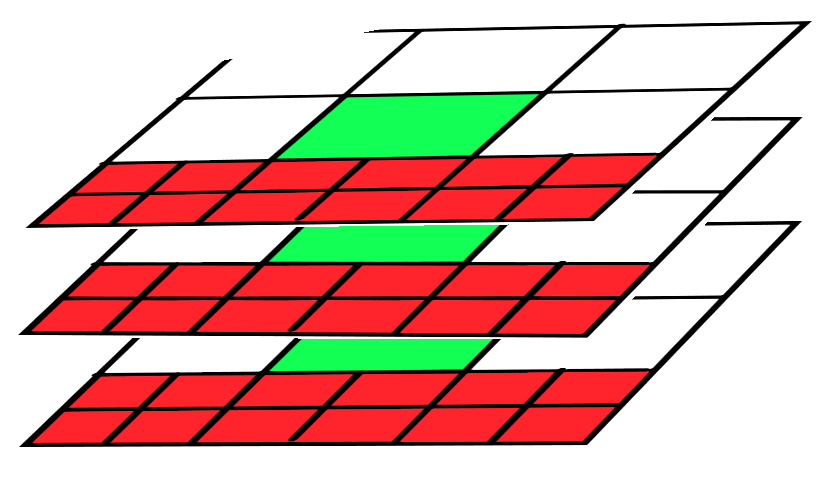
\includegraphics[width=4.5cm]{figures/met9max_mean.PNG}
    \caption{common figure for both max and mean}
    \label{fig:my_label}
\end{figure}

\end{enumerate}

\subsubsection{Annual maxima model intention}
1GRID is a plain selection method compared to the other methods. The initial reason for using other methods was that 1GRID was underestimating the resulting IDF-curves compared to the station-based curves for almost all stations and durations. 9GRID is designed to be an optimal selection method is the sense that the absolute maximum values possible for the area as an entity is chosen for each duration. This was to ensure that any event near the gridpoint in question also was captured. 9GRID is artificial compared to the others because a maximum value for any given duration may consist of precipitation values from different gridpoints, where the next maximum value may consist of entirely different gridpoint values. Whereas in 9GRID the annual maximum value for a given duration and year can originate from several gridpoints, in the 9MAX method it originates from one gridpoint. Thus, 9MAX appears more consistent with the station-based approach, or at least some sort of in-between solution to the station-based IDF-values and the 9GRID IDF-values. 9MEAN is a smooth version of the 9MAX. Since the mean annual maximum value out of the 9 gridpoints is used it should ensure an improved area-representation compared to 1GRID. However, as Figure 1 and Figure 2 displays, the IDF-value difference between 1GRID and 9MEAN is very small both for small and large return periods.    

\subsubsection{comment on AM methods}

The two "new"/other 9-grid based selection methods are built differently. Now the annual maximum value for each of the nine  gridpoints for each duration is extracted directly and put into a 3x3 matrix. Either maximum ($MAX$) or mean ($MEAN$)values of the nine is then calculated per duration to give a one-dimensional data series. The $MAX$ alternative is designed to be a less aggressive optimisation of the annual maximum values around the station compared to the other nine-grid maximum selection method \textbf{make a name for this one as well!}. The  $MAX$ maximization method is possibly closer to the real world compared to the \textbf{$XXX$} method. Extracting maximum value for each timestep out of the nine gridpoints might be artificial in one way, since the annual maxima for any duration may be composed from different locations. The $MAX$ method is on the other hand more realistic in the sens that the annul maxima for certain year always origins from one gridpoint. 
